To model the botnet under study, Mirai, with the final objective of performing our feasibility analysis, we first need to understand the Mirai infection process, all the entities involved in the process, and how these entities interact with each other. In this section, we detail the Mirai infection process and present our timed automata model of the Mirai botnet developed in UPPAAL.
% Mirai Infection Process
\begin{figure}[h!]
    \centering
    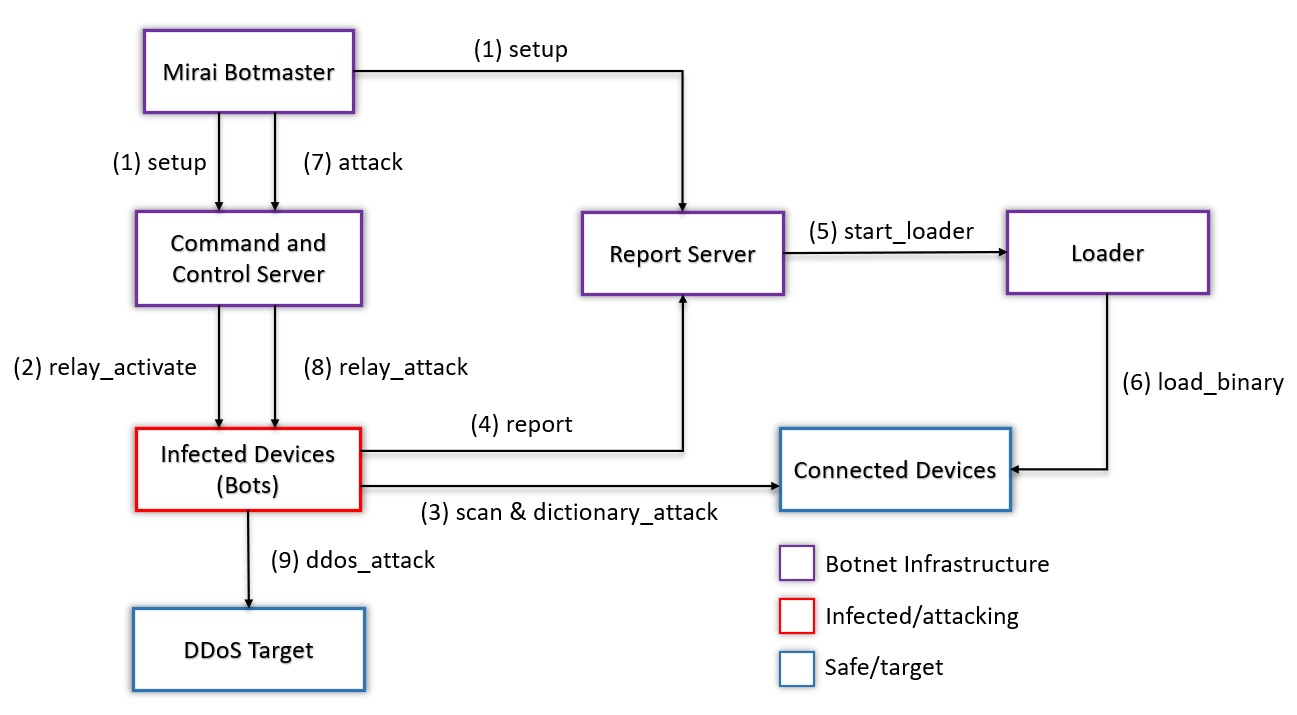
\includegraphics[width=\linewidth]{Figures/mirai_infection_process.jpg}
    \caption{Mirai Infection Process}
    \vspace{-0.2 cm}
    \label{fig:mirai_infection_process}
\end{figure}
\par


% Start Subsection**************************************************************************************
\subsection{Mirai Infection Process}
\label{sub:mirai_infection_process}
% ====================================== The entities involved =========================================
Mirai falls under the category of classical centralized botnets that revolve around a single central C\&C server to spread~\cite{shanmughapriya2018_botnet_of_things_survey}. Figure~\ref{fig:mirai_infection_process} illustrates the primary components of the centralized infrastructure (a C\&C server, a Report server, and a Loader) as well as the way these components interact. These entities are under the control of the Mirai botmaster, who actuates and directs the botnet activity through the infrastructure. The botnet is also comprised of the devices that have already been infected, also known as bots, that actively seek out other vulnerable connected devices in the network to infect. The bots under control can be further directed to compromise a DDoS target with a variety of DDoS attacks under Mirai's disposal~\cite{kambourakis2017mirai}.
\par
% ==================================== Steps: Mirai Infection Process ====================================
The Mirai infection process can be outlined in a number of simplified steps~\cite{kambourakis2017mirai, Antonakakis2017_USENIX_Mirai_First_Study}:
\begin{enumerate}
    \item The botmaster begins the infection process by setting up the remote C\&C server and the Report server.
    \item The C\&C server activates the first bot, one that is infected from the beginning, to initiate the scan-attack-report cycle of a bot.
    \item The bot statelessly scans the network for open Telnet ports at randomly selected IP addresses, and initiates a brute force remote-login attempt by randomly selecting 10 out of the 62 default or commonly used credentials hard-coded in the Mirai binary.
    \item If a brute force attack is successful, the attacking bot reports the victim \emph{id} (device IP and the credentials that worked) to the Report server.
    \item If the reported device is not part of the botnet, the report server adds it to its records, and subsequently, activates the Loader to load the malware binary into the new vulnerable device.
    \item The Loader determines the architecture of the target device and uploads a hardware-specific malware, transforming the target device into another bot. Steps 3 to 6 continue until the botnet is large enough for the attacker's purpose or about all the vulnerable devices in the network have been compromised.
    \item Any time, ideally with an adequately sized botnet, the botmaster can issue an attack command to the C\&C server.
    \item The C\&C server relays the attack command to all the bots that are currently under control.
    \item The bots stop their usual scan-attack-report cycle and start performing a DDoS and/or other malicious attacks on the attack target.
\end{enumerate}
% End Subsection******************************************************************************************



% Start Subsection****************************************************************************************
% ================================== Modeling the Botnet Infrastructure ==================================
\subsection{Modeling the Mirai Botnet Infrastructure}
\label{sub:modeling_botnet_infrastructure}
We start by modeling the key entities - the C\&C server, the Report server, and the Loader - in the Mirai botnet infrastructure. Each entity is modeled as a separate automaton that engages in multiple channel synchronizations to reflect the behavior of a botnet in a real-time network. For a brief discussion about the notations used extensively throughout the modeling process, please refer to section~\ref{sub: modeling_in_uppaal}.
% The CnC server automaton
\begin{figure}[H]
    \centering
    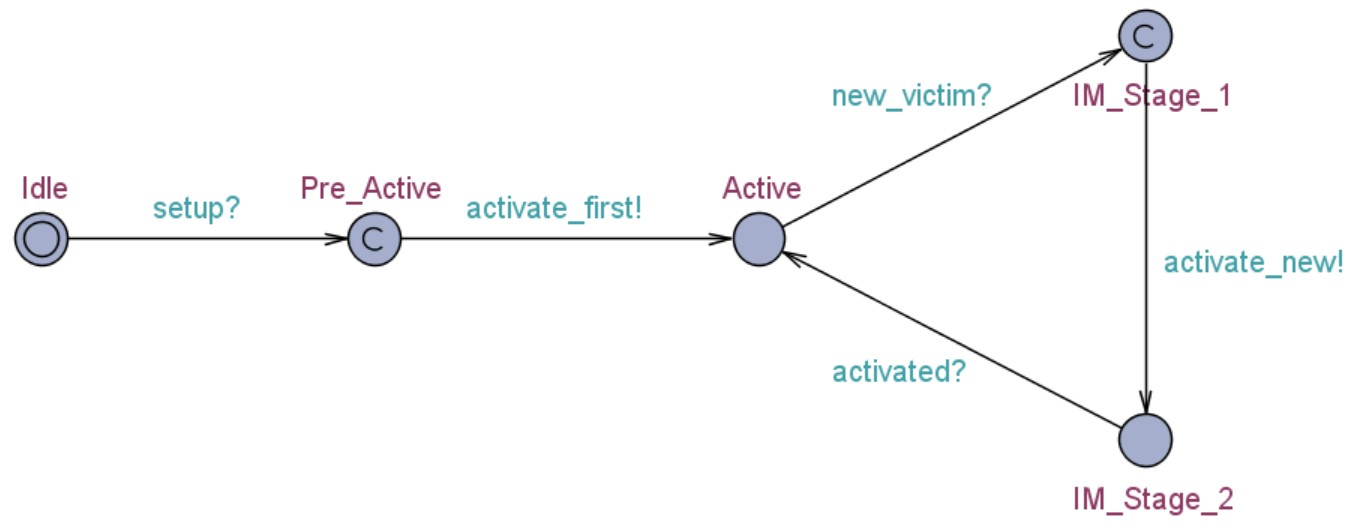
\includegraphics[width=\linewidth]{Figures/CnC_srv_automaton.jpg}
    \caption{The Command and Control Server Automaton (\CNC)}
    \vspace{-0.3 cm}
    \label{fig:CnC_server_automaton}
\end{figure}
\par
Figure~\ref{fig:CnC_server_automaton} presents the Command and Control server automaton (\CNC) with its two primary states \state{Idle} and \state{Active}. The server is set up by the abstract Mirai botmaster entity, after which \CNC activates the first bot (pre-infected) and transitions to its \state{Active} state. In this state, \CNC waits for raw socket connections from new victims, only to activate them later so they can start their own infection process.
% The Report server automaton
\begin{figure}[h!]
    \centering
    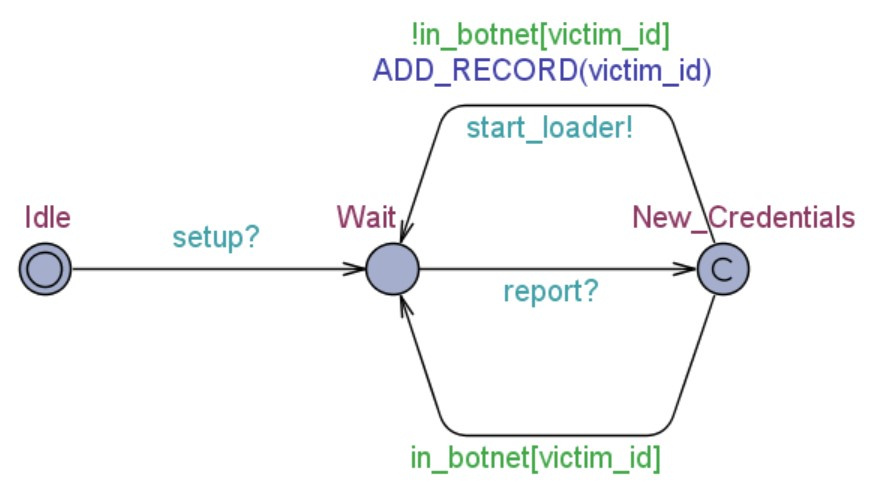
\includegraphics[width=.65\linewidth]{Figures/Report_srv_automaton.jpg}
    \caption{The Report Server Automaton (\RPT)}
    \vspace{-0.1 cm}
    \label{fig:report_server_automaton}
\end{figure}
\par
Figure~\ref{fig:report_server_automaton} illustrates the behavior of the Report server automaton (\RPT). Similar to \CNC, \RPT is also set up the Mirai botmaster, allowing the transition from the \state{Idle} state to the \state{Wait} state. Once in the \state{Wait} state, the \RPT listens for incoming reports of a new victim \emph{id} sent via each bot on port 80 every minute. Any new \emph{id} is checked against the current records. \LDR adds a new record as well as activates the Loader automaton if the \emph{id} proves to be a vulnerable device that is yet to be infected.
% The Loader automaton
\begin{figure}[h!]
    \centering
    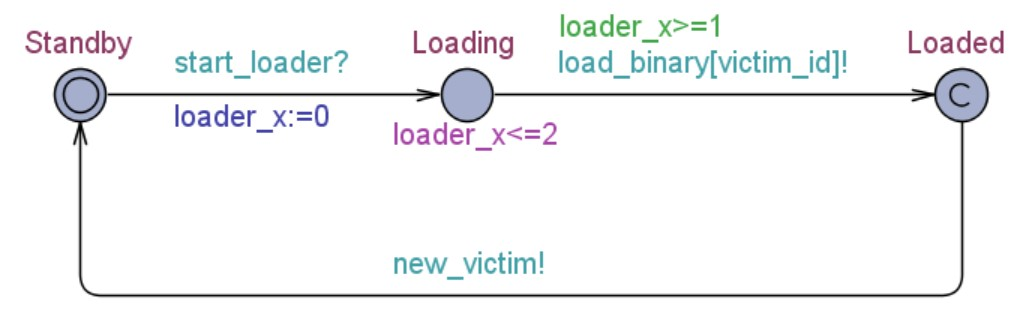
\includegraphics[width=.8\linewidth]{Figures/Loader_automaton.jpg}
    \caption{The Loader Automaton (\LDR)}
    \vspace{-0.1 cm}
    \label{fig:loader_automaton}
\end{figure}
\par
% The image is here only for formatting purposes
% Device type 1 - Always Connected
\begin{figure*}[t!]
    \centering
    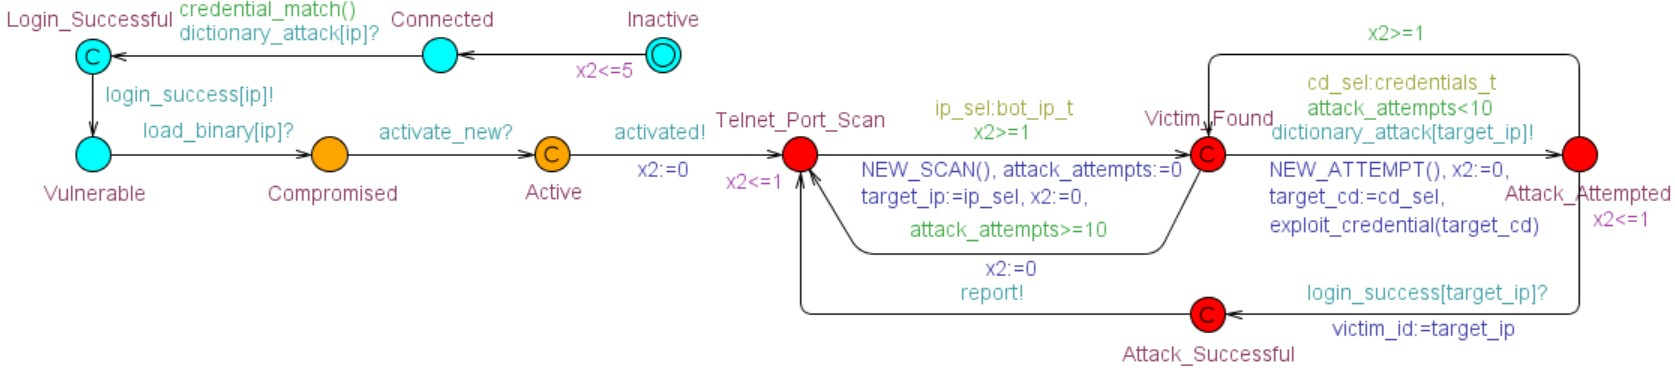
\includegraphics[width=\linewidth]{Figures/Device_t1_automaton.jpg}
    \caption{Device Automaton A (\DA) - Always-Connected}
    \vspace{-0.1 cm}
    \label{fig:device_type_a}
\end{figure*}
\par
Figure~\ref{fig:loader_automaton} shows the Loader automaton (\LDR) that reflects the inner workings of the proxies called loaders~\cite{kambourakis2017mirai}. \LDR moves from its initial \state{Standby} state to the \state{Loading} state after it has received the start\_loader command from the report server along with a vulnerable victim \emph{id}. In the \state{Loading} state, \LDR takes anywhere between one to two time units to log into the victim using the provided \emph{id} and instructs the victim to download and execute the hardware-appropriate binary, essentially turning the victim into a functional bot. After this process is over, \LDR informs \CNC about this new botnet member and returns to its \state{Standby} state.
% End Subsection******************************************************************************************



% Start Subsection****************************************************************************************
\subsection{Modeling Always-Connected Devices}
\label{sub:modeling_always_connected_devices}
After the botnet infrastructure, we focus our attention on modeling the individual device behavior inside the botnet. The device behavior here refers to the behavior when the device acts as a normal device as well as when the device is infected and being used by the botmaster for their nefarious purposes. Figure~\ref{fig:device_type_a} shows our first device automaton (\DA) where the states involved in the three different modes of behavior - (1) when the device behaves like a regular device,  (2) when it is being infected, as well as (3) when it is acting as a bot - are marked in colors blue, orange, and red, respectively.
\par
% =========================================== The device mode =============================================
\AC devices, according to RFC 7228, are representative of IoT devices that are always-on (P9) and stay connected to the network all the time~\cite{RFC_7228}. All the states marked in blue represent the regular and intended behavior of a device. \DA starts in the \state{Inactive} state and connects to the network after a specific time (within five time units of the simulation start in our model), moving to its \state{connected} state. This is the only state where another \DA in their infected mode (red) can perform dictionary attacks on a \DA. If an attack is performed with a matching credential, then \DA moves to its \state{vulnerable} state where it now has its \emph{id} leaked to the report server.
\par
% ==================================== The transition into a bot phase ====================================
States depicted in Orange represent the transition state of a device during its infection process. In the \state{Vulnerable} state, the device can be logged in to download the Mirai binary into the device. Once this process is complete, \DA moves to the compromised state, where it waits to establish a raw socket connection with the C\&C server to receive further commands. After establishing the connection, \DA moves to the \state{Telnet\_Port\_Scan} state where it now starts to act upon the commands relayed by the C\&C server.
% ========================================= The infected mode: bot ========================================
The red states in the right portion of \DA represent the same device's behavior once it is infected, activated, and has started performing activities befitting that of a bot. In the \state{Telnet\_Port\_Scan} state, the infected device now statelessly scans the network for pseudorandom IPv4 addresses for open Telnet 23 ports, and once found, moves to the \state{Victim\_Found} state. This is the state where a bot tries to gain a working Linux shell, attempting to randomly select and use 10 out of 62 hardcoded default or commonly used credentials stored in the original Mirai binary~\cite{kambourakis2017mirai}. An unsuccessful attack chain of ten takes the bot back to the \state{Telnet\_Port\_Scan} state, whereas a successful attack leads to the \state{Attack\_Successful} state first, where the victim information is reported to the Report server.
\par
% ====================================== IF space: talk about timing ======================================
% End Subsection******************************************************************************************


% Start Subsection****************************************************************************************
\subsection{Modeling Reboot-Capable Devices}
\label{sub:modeling_reboot_capable_devices}
Next, we model the behavior of devices that are capable of rebooting and reconnecting to the network once rebooted. This capability is crucial as the Mirai binary is stored in the dynamic memory and is cleared once an infected device is rebooted, essentially restoring the regular device behavior~\cite{tanaka2019_PN_Botnet}. To introduce rebooting to our device automaton, we present a modified automaton in figure~\ref{fig:device_type_b} with this capability.
\par
% The image is here only for formatting purposes
% Device type 2 - Reboot Capable
\begin{figure*}[t!]
    \centering
    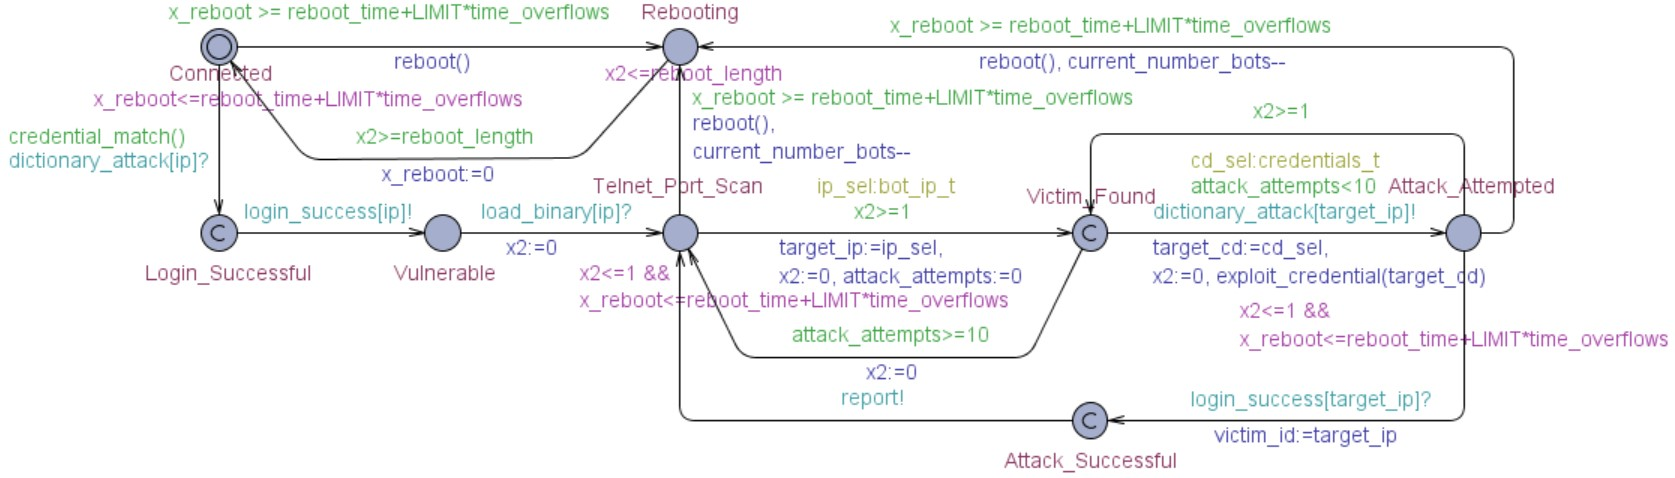
\includegraphics[width=\linewidth]{Figures/Device_t2_automaton.jpg}
    \caption{Device Automaton B (\DB) - Reboot-Capable}
    \label{fig:device_type_b}
    \vspace{-0.3 cm}
\end{figure*}
\par

% ======================================= Device Clusters: Reboot =========================================
Our second device automaton (\DB) represents clusters of \RC devices that can reboot either periodically or manually with user intervention. One particular example of this would be router configurations that allow a router to preserve its health by turning off for an hour each day when not under use. Devices of category E1 (battery-powered devices with a fixed primary battery replacement interval) and P0 (normally turned off, only attached to the network when needed), also fall under the same category and can be modeled with simple attunement of the timing constraints~\cite{RFC_7228}.
\par
% ======================================== The Reboot Capability ==========================================
\DB is extended with two new adjustable parameters for rebooting. Each device of type \DB now starts with a \emph{reboot\_time} that represents a predetermined time after which each device will turn off, moving to the \state{Rebooting} state regardless of its infection status. Additionally, another parameter, \emph{reboot\_length}, determines how much time a device takes to reboot and/or the time a device stays off after turning off. These parameters can be adjusted all at once or manually before each simulation, and the fact that we can represent stochastic timing behavior gives us great flexibility in modeling the various device clusters mentioned before. Moreover, this lets us model different distributions of various devices of type \DB, or \DA and \DB combined, and allows us to extend the model with other device automatons (e.g., with patching capability) in the future.
% End Subsection******************************************************************************************